\documentclass[a4paper,12pt]{article}%
\usepackage[T1]{fontenc}%
\usepackage[utf8]{inputenc}%
\usepackage{lmodern}%
\usepackage{textcomp}%
\usepackage{lastpage}%
\usepackage{graphicx}%
%

\usepackage[left=1.5cm,right=1.5cm,top=2cm,bottom=2cm]{geometry}
\usepackage{setspace}
\onehalfspacing
\usepackage[portuguese]{babel}
\usepackage{caption}
\usepackage{amsmath}
\usepackage{cals, ragged2e}
\usepackage{breqn}
\usepackage{pdflscape}
\usepackage{multicol}
\usepackage[colorlinks=true,linkcolor=black,anchorcolor=black,citecolor=black,filecolor=black,menucolor=black,runcolor=black,urlcolor=black]{hyperref}
\usepackage{float}
\usepackage{gensymb}
\usepackage{fancyhdr}
\pagestyle{fancy}
\fancyhf{}
\rhead{
\includegraphics[width=0.05\textwidth]{figs/logo.png}}
\lhead{Structures Explained}
\cfoot{\thepage}
\renewcommand{\footrulewidth}{0.4pt}
\usepackage[scaled=1]{helvet}
\renewcommand{\familydefault}{\sfdefault}
%
%
\begin{document}%
\normalsize%

            \begin{titlepage}
            
            \newcommand{\HRule}{\rule{\linewidth}{0.5mm}}
            
            \center
            
            
\includegraphics[width=0.75\textwidth]{figs/logo.png}\\[1cm]
            \vspace{\fill}
            {\LARGE Structures Explained\\ Resolução da Estrutura}\\[1.5cm]
            
            \HRule \\[0.6cm]
            
                 \large\textbf{Laboratório AeroTech}\\[0.5cm]
                 \large\textbf{Departamento de Engenharia Aeronáutica}\\[0.5cm]
                 \textsc{\Large Universidade de São Paulo}\\[0.5cm]
                 
             \HRule \\[1.5cm]            
            
             \vfill
        
             \end{titlepage}
        
             \newpage
             %
\section{Imagem da Estrutura}%
\label{sec:ImagemdaEstrutura}%


\begin{figure}[H]%
\centering%
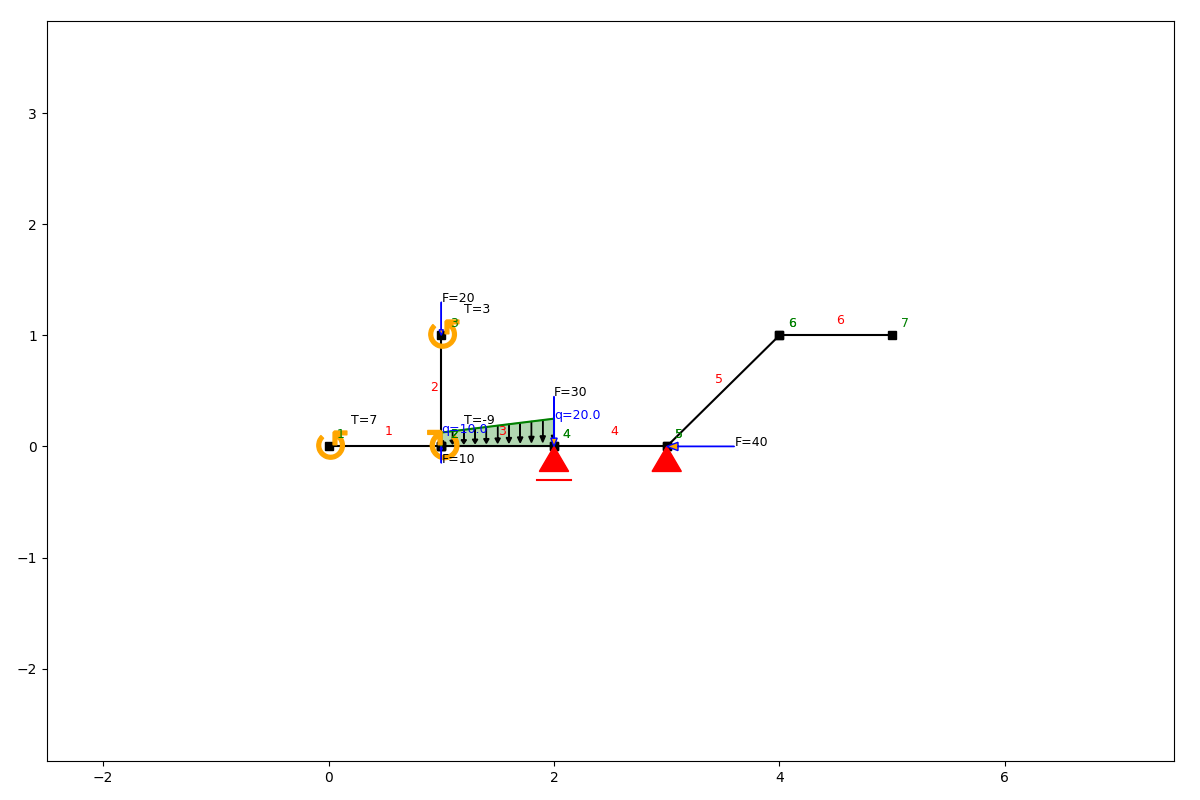
\includegraphics[width=500px]{figs/structure}%
\caption{\label{fig:estrutura} Imagem da estrutura com apoios e carregamentos}%
\end{figure}

%
\section{Fazendo o diagrama de corpo livre}%
\label{sec:Fazendoodiagramadecorpolivre}%


\begin{figure}[H]%
\centering%
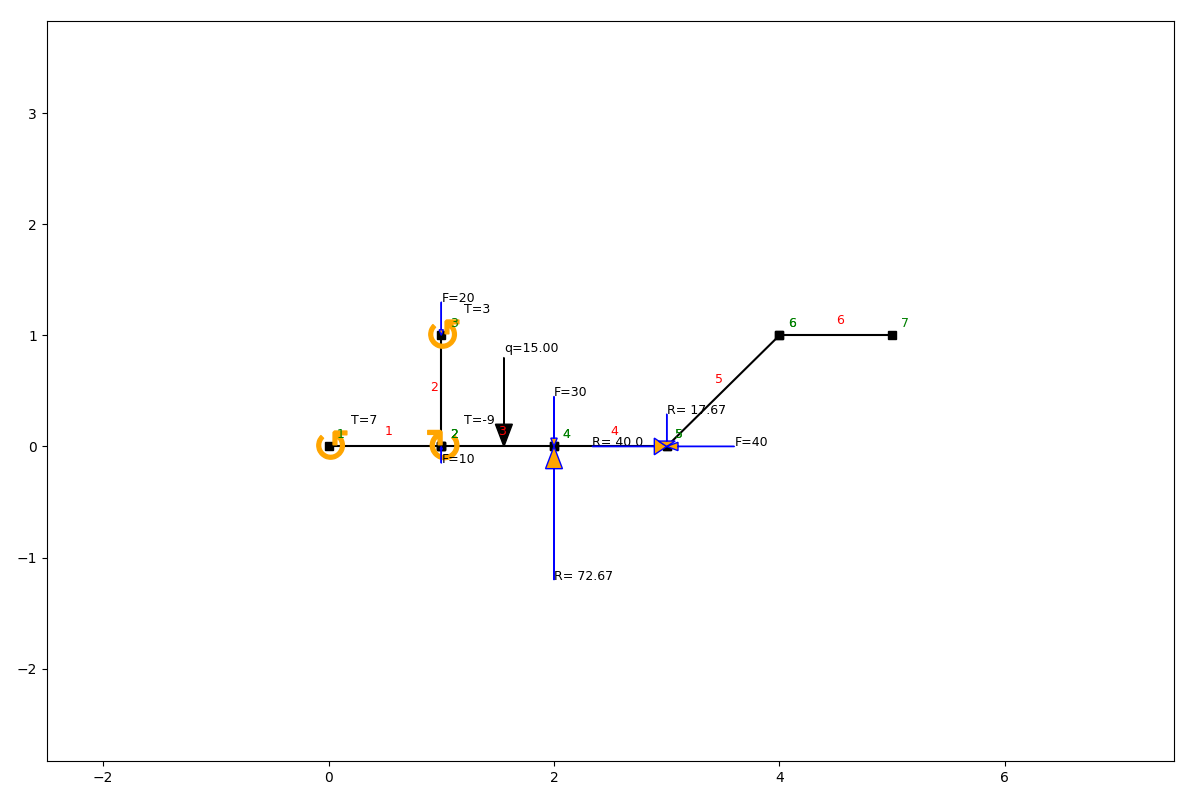
\includegraphics[width=500px]{figs/diagram1}%
\caption{\label{fig:corpolivre} Diagrama de corpo livre}%
\end{figure}

%
\section{Calculando a reação dos apoios}%
\label{sec:Calculandoareaodosapoios}%
\subsection{Realizando cálculo do momento no apoio fixo}%
\label{subsec:Realizandoclculodomomentonoapoiofixo}%
\begin{dmath*}%
\sum{M} = 0 \\%
\end{dmath*}%
\begin{dmath*}%
M = F \cdot d%
\end{dmath*}%
\begin{dmath*}%
j \left(-20.0\right) 2.0 i + j \left(-30.0\right) 1.0 i + j \left(-15.0\right) 1.44 i + j 10.0 \cdot 2.0 i + k \left(-9.0\right) + 3.0 k + 7.0 k - By \cdot i \left(-1.0\right) = 0 \\%
\end{dmath*}%
\begin{dmath*}%
By = 72.67k$ $N%
\end{dmath*}

%
\section{Refazendo o diagrama de corpo livre}%
\label{sec:Refazendoodiagramadecorpolivre}%


\begin{figure}[H]%
\centering%
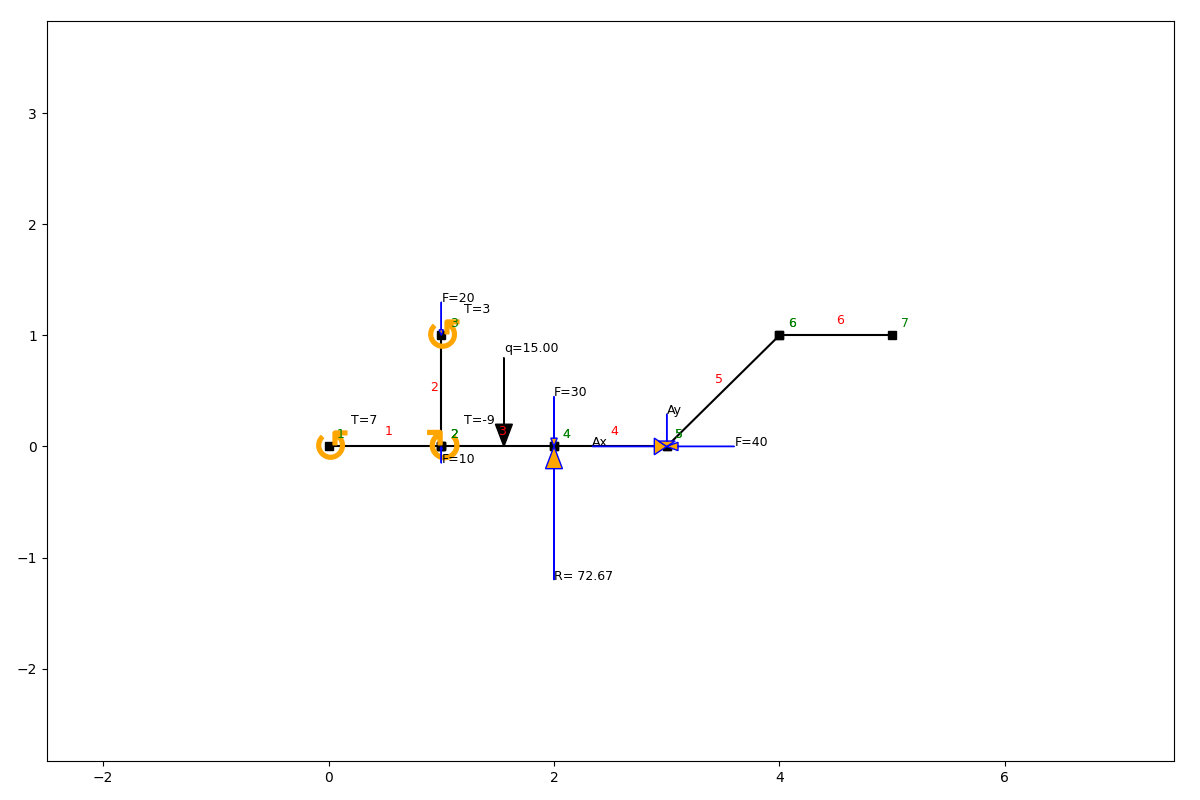
\includegraphics[width=500px]{figs/diagram2}%
\caption{\label{fig:corpolivre} Diagrama de corpo livre}%
\end{figure}

%
\subsection{Fazendo a somatória das forças em Y para obter a reação em Y no apoio fixo}%
\label{subsec:FazendoasomatriadasforasemYparaobterareaoemYnoapoiofixo}%
\begin{dmath*}%
\sum{Fy} = 0 \\%
\end{dmath*}%
\begin{dmath*}%
-30.0 - 20.0 - 15.0 + 10.0 + 72.67 - Ay = 0\\%
\end{dmath*}%
\begin{dmath*}%
Ay = 17.67$ $N%
\end{dmath*}

%
\subsection{Fazendo a somatória das forças em X para obter a reação em X no apoio fixo}%
\label{subsec:FazendoasomatriadasforasemXparaobterareaoemXnoapoiofixo}%
\begin{dmath*}%
\sum{Fx} = 0 \\%
\end{dmath*}%
\begin{dmath*}%
-40.0 + Ax = 0\\%
\end{dmath*}%
\begin{dmath*}%
Ax = 40.0$ $N%
\end{dmath*}

%
\subsection{Desenhando as reações dos apoios}%
\label{subsec:Desenhandoasreaesdosapoios}%


\begin{figure}[H]%
\centering%
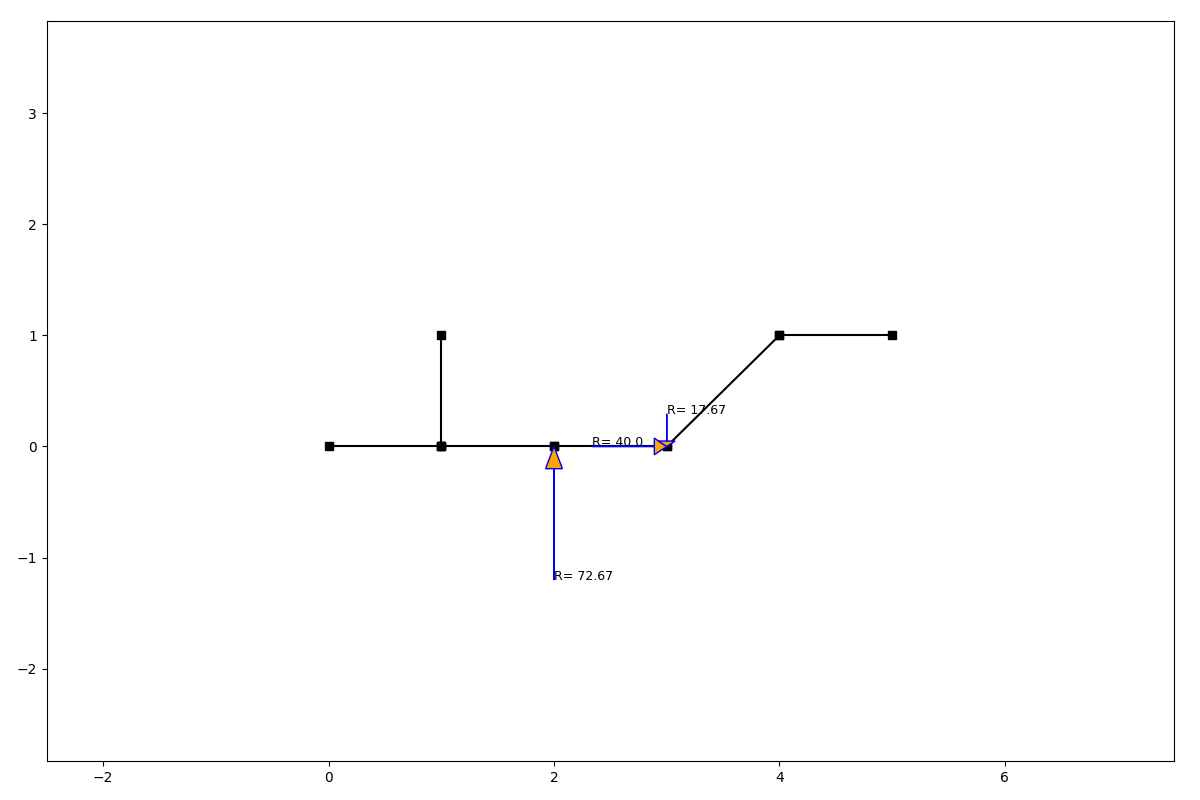
\includegraphics[width=500px]{figs/supports}%
\caption{\label{fig:apoios} Reações dos apoios}%
\end{figure}

%
\section{Calculando os esforços internos}%
\label{sec:Calculandoosesforosinternos}%
A partir da integral da força cortante, é obtido o momento fletor.%
\linebreak%
A constante de integração será o momento no nó final da seção anterior.%
\linebreak%
\subsection{Cortando na Seção 1}%
\label{subsec:CortandonaSeo1}%


\begin{figure}[H]%
\centering%
\includegraphics[width=500px]{figs/structure1}%
\caption{\label{fig:secoes}\label{fig:secoes} 1}%
\end{figure}

%
\subsubsection{Força Normal}%
\label{ssubsec:ForaNormal}%
\begin{dmath*}%
\sum{Fx} = 0 \\%
\end{dmath*}%
\begin{dmath*}%
0 + N = 0%
\end{dmath*}%
\begin{dmath*}%
N = 0$ $N%
\end{dmath*}

%
\subsubsection{Força Cortante}%
\label{ssubsec:ForaCortante}%
\begin{dmath*}%
\sum{Fy} = 0 \\%
\end{dmath*}%
\begin{dmath*}%
0 - V = 0%
\end{dmath*}%
\begin{dmath*}%
V = 0$ $N%
\end{dmath*}

%
\subsubsection{Momento Fletor}%
\label{ssubsec:MomentoFletor}%
\begin{dmath*}%
M = \int0 dx%
\end{dmath*}%
Need to sum moment at beginning of section to constant%
\begin{dmath*}%
c = c + +7.0%
\end{dmath*}%
\begin{dmath*}%
M = 7.0$ $N \cdot m%
\end{dmath*}

%
\subsection{Cortando na Seção 2}%
\label{subsec:CortandonaSeo2}%


\begin{figure}[H]%
\centering%
\includegraphics[width=500px]{figs/structure2}%
\caption{\label{fig:secoes}\label{fig:secoes} 2}%
\end{figure}

%
\subsubsection{Força Normal}%
\label{ssubsec:ForaNormal}%
\begin{dmath*}%
\sum{Fx} = 0 \\%
\end{dmath*}%
\begin{dmath*}%
-20.0 + N = 0%
\end{dmath*}%
\begin{dmath*}%
N = -20.0$ $N%
\end{dmath*}

%
\subsubsection{Força Cortante}%
\label{ssubsec:ForaCortante}%
\begin{dmath*}%
\sum{Fy} = 0 \\%
\end{dmath*}%
\begin{dmath*}%
0 - V = 0%
\end{dmath*}%
\begin{dmath*}%
V = 0$ $N%
\end{dmath*}

%
\subsubsection{Momento Fletor}%
\label{ssubsec:MomentoFletor}%
\begin{dmath*}%
M = \int0 dx%
\end{dmath*}%
Need to sum moment at beginning of section to constant%
\begin{dmath*}%
c = c + +3.0%
\end{dmath*}%
\begin{dmath*}%
M = 3.0$ $N \cdot m%
\end{dmath*}

%
\subsection{Cortando na Seção 3}%
\label{subsec:CortandonaSeo3}%


\begin{figure}[H]%
\centering%
\includegraphics[width=500px]{figs/structure3}%
\caption{\label{fig:secoes}\label{fig:secoes} 3}%
\end{figure}

%
\subsubsection{Força Normal}%
\label{ssubsec:ForaNormal}%
\begin{dmath*}%
\sum{Fx} = 0 \\%
\end{dmath*}%
\begin{dmath*}%
0 + N = 0%
\end{dmath*}%
\begin{dmath*}%
N = 0$ $N%
\end{dmath*}

%
\subsubsection{Força Cortante}%
\label{ssubsec:ForaCortante}%
\begin{dmath*}%
\sum{Fy} = 0 \\%
\end{dmath*}%
\begin{dmath*}%
- 10.0 x + x^{2.0} \left(-5.0\right) - 20.0 + 10.0 - V = 0%
\end{dmath*}%
\begin{dmath*}%
V = - 10.0 x - 5.0 x^{2.0} - 10.0$ $N%
\end{dmath*}

%
\subsubsection{Momento Fletor}%
\label{ssubsec:MomentoFletor}%
\begin{dmath*}%
M = \int- 10.0 x - 5.0 x^{2.0} - 10.0 dx%
\end{dmath*}%
\begin{dmath*}%
c(x) = +-1.11676628463617e-15*x**2 + 8.65827297282269e-16*x - 3.0%
\end{dmath*}%
\begin{dmath*}%
c(1.0) = -3.00000000000000%
\end{dmath*}%
Need to sum moment at beginning of section to constant%
\begin{dmath*}%
c = c + +-9.0%
\end{dmath*}%
\begin{dmath*}%
M = - 10.0 x - 5.0 x^{2.0} - 1.67 x^{3.0} - 12.0$ $N \cdot m%
\end{dmath*}

%
\subsection{Cortando na Seção 4}%
\label{subsec:CortandonaSeo4}%


\begin{figure}[H]%
\centering%
\includegraphics[width=500px]{figs/structure4}%
\caption{\label{fig:secoes}\label{fig:secoes} 4}%
\end{figure}

%
\subsubsection{Força Normal}%
\label{ssubsec:ForaNormal}%
\begin{dmath*}%
\sum{Fx} = 0 \\%
\end{dmath*}%
\begin{dmath*}%
0 + N = 0%
\end{dmath*}%
\begin{dmath*}%
N = 0$ $N%
\end{dmath*}

%
\subsubsection{Força Cortante}%
\label{ssubsec:ForaCortante}%
\begin{dmath*}%
\sum{Fy} = 0 \\%
\end{dmath*}%
\begin{dmath*}%
-30.0 - 20.0 - 15.0 + 10.0 + 72.67 - V = 0%
\end{dmath*}%
\begin{dmath*}%
V = 17.67$ $N%
\end{dmath*}

%
\subsubsection{Momento Fletor}%
\label{ssubsec:MomentoFletor}%
\begin{dmath*}%
M = \int17.67 dx%
\end{dmath*}%
\begin{dmath*}%
c(x) = +7.49999999999999*x**2 + 9.01006525058998*x + 1.07830070803834%
\end{dmath*}%
\begin{dmath*}%
c(1.0) = 17.5883659586283%
\end{dmath*}%
\begin{dmath*}%
M = 17.67 x + 17.59$ $N \cdot m%
\end{dmath*}

%
\subsection{Cortando na Seção 5}%
\label{subsec:CortandonaSeo5}%


\begin{figure}[H]%
\centering%
\includegraphics[width=500px]{figs/structure5}%
\caption{\label{fig:secoes}\label{fig:secoes} 5}%
\end{figure}

%
\subsubsection{Força Normal}%
\label{ssubsec:ForaNormal}%
\begin{dmath*}%
\sum{Fx} = 0 \\%
\end{dmath*}%
\begin{dmath*}%
\left(-40.0 + 40.0\right) \cos{\left(315.0 ^\circ \right)} + N = 0%
\end{dmath*}%
\begin{dmath*}%
N = 0$ $N%
\end{dmath*}

%
\subsubsection{Força Cortante}%
\label{ssubsec:ForaCortante}%
\begin{dmath*}%
\sum{Fy} = 0 \\%
\end{dmath*}%
\begin{dmath*}%
0 - V = 0%
\end{dmath*}%
\begin{dmath*}%
V = 0$ $N%
\end{dmath*}

%
\subsubsection{Momento Fletor}%
\label{ssubsec:MomentoFletor}%
\begin{dmath*}%
M = \int0 dx%
\end{dmath*}%
\begin{dmath*}%
c(x) = +-3.27107385319014e-14*x**2 - 17.6666666666666*x + 17.6666666666667%
\end{dmath*}%
\begin{dmath*}%
c(1.0) = 6.67652444745126e-14%
\end{dmath*}%
\begin{dmath*}%
M = 0$ $N \cdot m%
\end{dmath*}

%
\subsection{Cortando na Seção 6}%
\label{subsec:CortandonaSeo6}%


\begin{figure}[H]%
\centering%
\includegraphics[width=500px]{figs/structure6}%
\caption{\label{fig:secoes}\label{fig:secoes} 6}%
\end{figure}

%
\subsubsection{Força Normal}%
\label{ssubsec:ForaNormal}%
\begin{dmath*}%
\sum{Fx} = 0 \\%
\end{dmath*}%
\begin{dmath*}%
-40.0 + 40.0 + N = 0%
\end{dmath*}%
\begin{dmath*}%
N = 0$ $N%
\end{dmath*}

%
\subsubsection{Força Cortante}%
\label{ssubsec:ForaCortante}%
\begin{dmath*}%
\sum{Fy} = 0 \\%
\end{dmath*}%
\begin{dmath*}%
-30.0 - 20.0 - 17.67 - 15.0 + 10.0 + 72.67 - V = 0%
\end{dmath*}%
\begin{dmath*}%
V = 0$ $N%
\end{dmath*}

%
\subsubsection{Momento Fletor}%
\label{ssubsec:MomentoFletor}%
\begin{dmath*}%
M = \int0 dx%
\end{dmath*}%
\begin{dmath*}%
c(x) = +2.48031971758904e-30*x**2 + 3.14018497110952e-15*x - 4.44089209850063e-15%
\end{dmath*}%
\begin{dmath*}%
c(1.4142135381698608) = -9.23885702859559e-30%
\end{dmath*}%
\begin{dmath*}%
M = 0$ $N \cdot m%
\end{dmath*}

%
\section{Desenhando os diagramas de esforços internos}%
\label{sec:Desenhandoosdiagramasdeesforosinternos}%
\subsection{Desenhando o diagrama da força normal:}%
\label{subsec:Desenhandoodiagramadaforanormal}%


\begin{figure}[H]%
\centering%
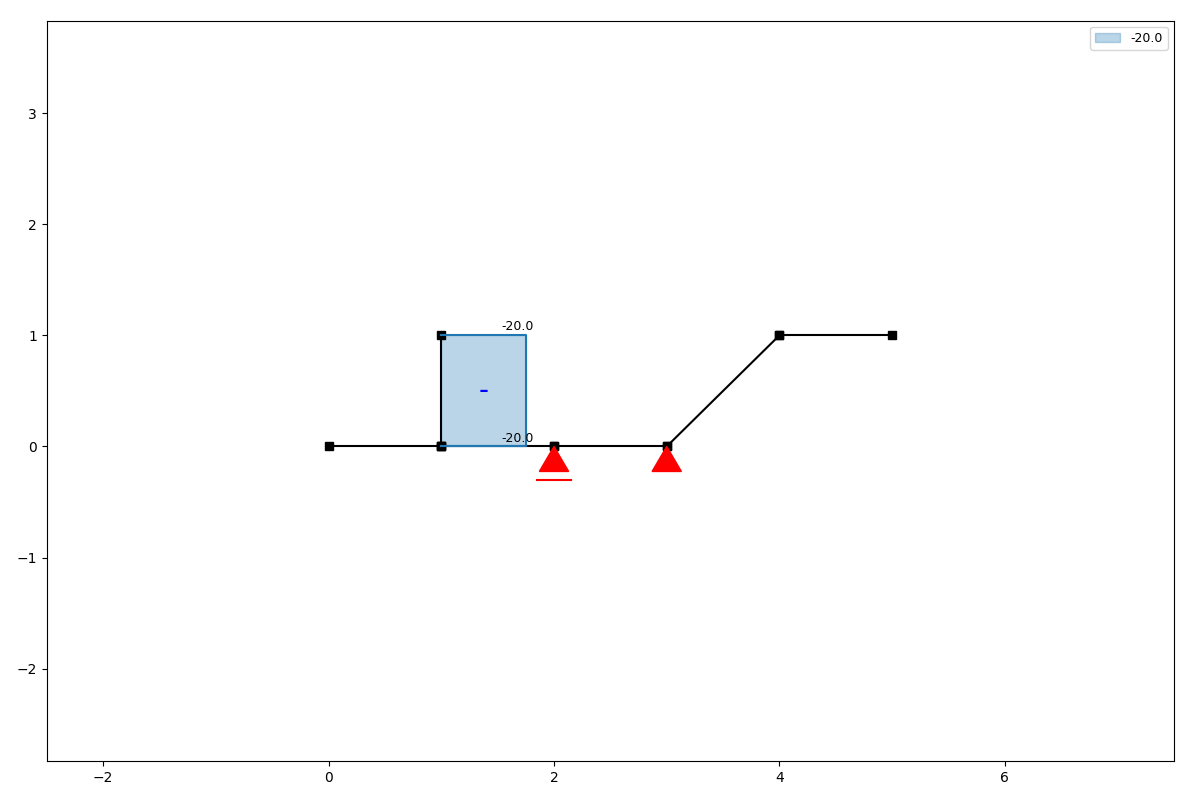
\includegraphics[width=500px]{figs/axial}%
\caption{\label{fig:normais} Força normal}%
\end{figure}

%
\subsection{Desenhando o diagrama da força cortante:}%
\label{subsec:Desenhandoodiagramadaforacortante}%


\begin{figure}[H]%
\centering%
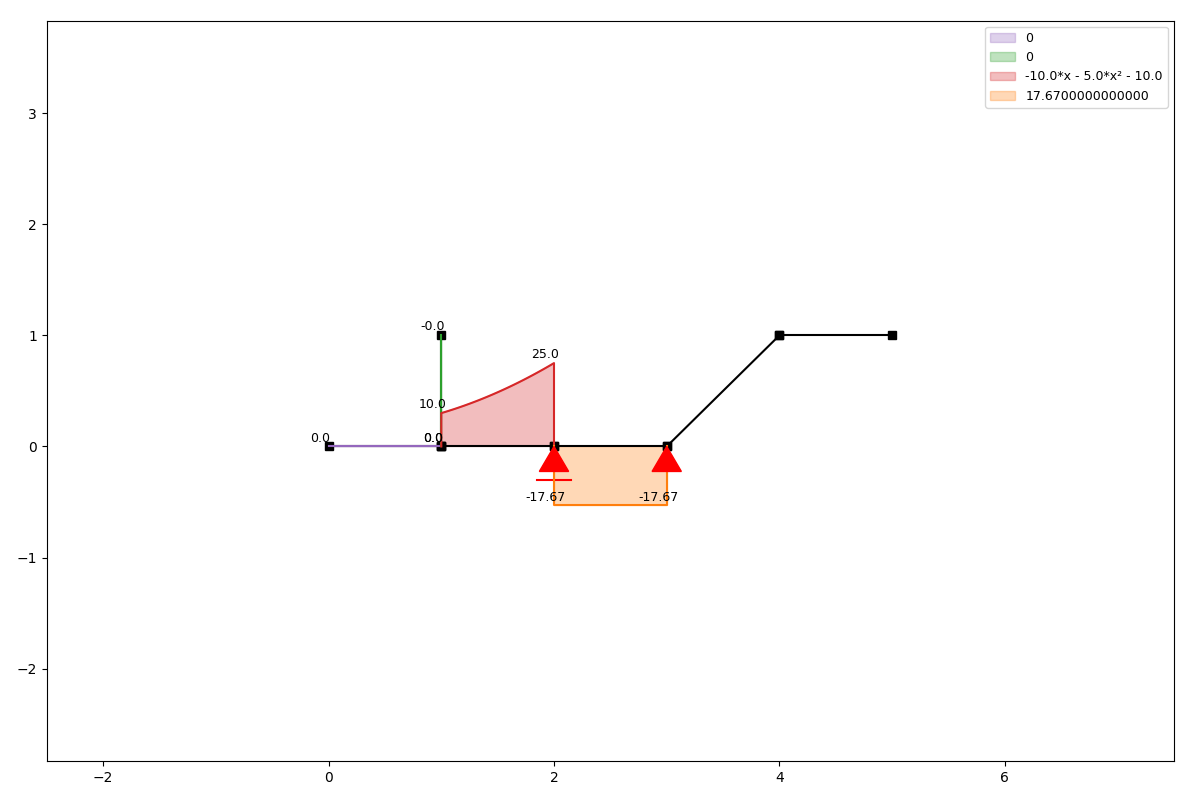
\includegraphics[width=500px]{figs/shear}%
\caption{\label{fig:cortante} Força cortante}%
\end{figure}

%
\subsection{Desenhando o diagrama do momento fletor:}%
\label{subsec:Desenhandoodiagramadomomentofletor}%


\begin{figure}[H]%
\centering%
\includegraphics[width=500px]{figs/moment}%
\caption{\label{fig:momento} Momento Fletor}%
\end{figure}

%
\end{document}